\chapter{Examples}  %3

Some examples of the definitions found in the file ps-defs.tex follow below.

%
%%%%%%%%%%%%%%%%%%%%%%%%%%%%%%%%%%%%%%%%%%%
%	EXAMPLES follow below
%%%%%%%%%%%%%%%%%%%%%%%%%%%%%%%%%%%%%%%%%%%
%%%%%%%%%%%%%%%%%%%%%%%%%%%%%%%%%%%%%%%%%%%%%%%%%
%%  Below are 3 examples of similar equations
%%        using equation numbers or not.
%%%%%%%%%%%%%%%%%%%%%%%%%%%%%%%%%%%%%%%%%%%%%%%%%
Here are examples of how you can use equation numbers with multiple line equations.
\begin{align}			%Eqn number on more than one line
(f+(g+h))(a)&=f(a)+(g+h)(a)  \nonumber \\
& =f(a)+(g(a)+h(a))   \\
& =(f(a)+g(a))+h(a)  \nonumber \\
& = (f+g)(a)+h(a)  \nonumber \\
& =((f+g)+h)(a)
\end{align}
%
\begin{equation}			%Eqn number centered on equations
\begin{aligned}
(f+(g+h))(a)&=f(a)+(g+h)(a)  \\
& =f(a)+(g(a)+h(a))  \\
& =(f(a)+g(a))+h(a)   \\
& = (f+g)(a)+h(a)   \\
& =((f+g)+h)(a)	
\end{aligned}
\end{equation}  
%
\[					%No equation number
\begin{aligned}			
(f+(g+h))(a)&=f(a)+(g+h)(a)\\
& =f(a)+(g(a)+h(a))\\
& =(f(a)+g(a))+h(a)\\
& = (f+g)(a)+h(a)\\
& =((f+g)+h)(a)
\end{aligned}
\]

Below is a figure which shows how to line up small figures on multiple lines.
The .dvi version is immediately below.  The .pdf version may be found underneath the complete figure and commented out.  If you exchange the sections commented out, then you can compile a .pdf file. \\ 

%
\begin{figure}[h] %  Fig 3.1            % DVI version
\[
\begin{gathered}
\hbox to 1in{
\includegraphics[width=1in]{ch3-square.ps}}
\quad
\hbox to 1in{
\includegraphics[width=1in]{ch3-circle.ps}} \\
\hbox to 1in{\hfill(a)\hfill} \quad \hbox to 1in{\hfill(b)\hfill}
\end{gathered}
\]
%
\vskip 12pt			% vertical space between rows
\[
\begin{gathered}
\hbox to 1in{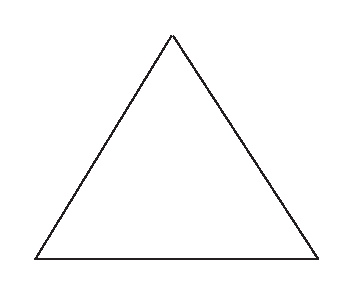
\includegraphics[width=1in]{ch3-triangle.ps}}\\
\hbox to 1in{\hfill(c)\hfill}
\end{gathered}
\]

\caption{Two rows of graphics: (a)~Square \ (b)~Circle \ (c)~Rectangle }\label{fig:3.1}
\end{figure}
%

%
%\begin{figure}[h] %  Fig 3.1                 % PDF version
%\[
%\begin{gathered}
%\hbox to 1in{
\includegraphics[width=1in]{ch3-square.pdf}}
%\quad
%\hbox to 1in{
\includegraphics[width=1in]{ch3-circle.pdf}} \\
%\hbox to 1in{\hfill(a)\hfill} \quad \hbox to 1in{\hfill(b)\hfill}
%\end{gathered}
%\]
%%
%\vskip 12pt			% vertical space between rows
%\[
%\begin{gathered}
%\hbox to 1in{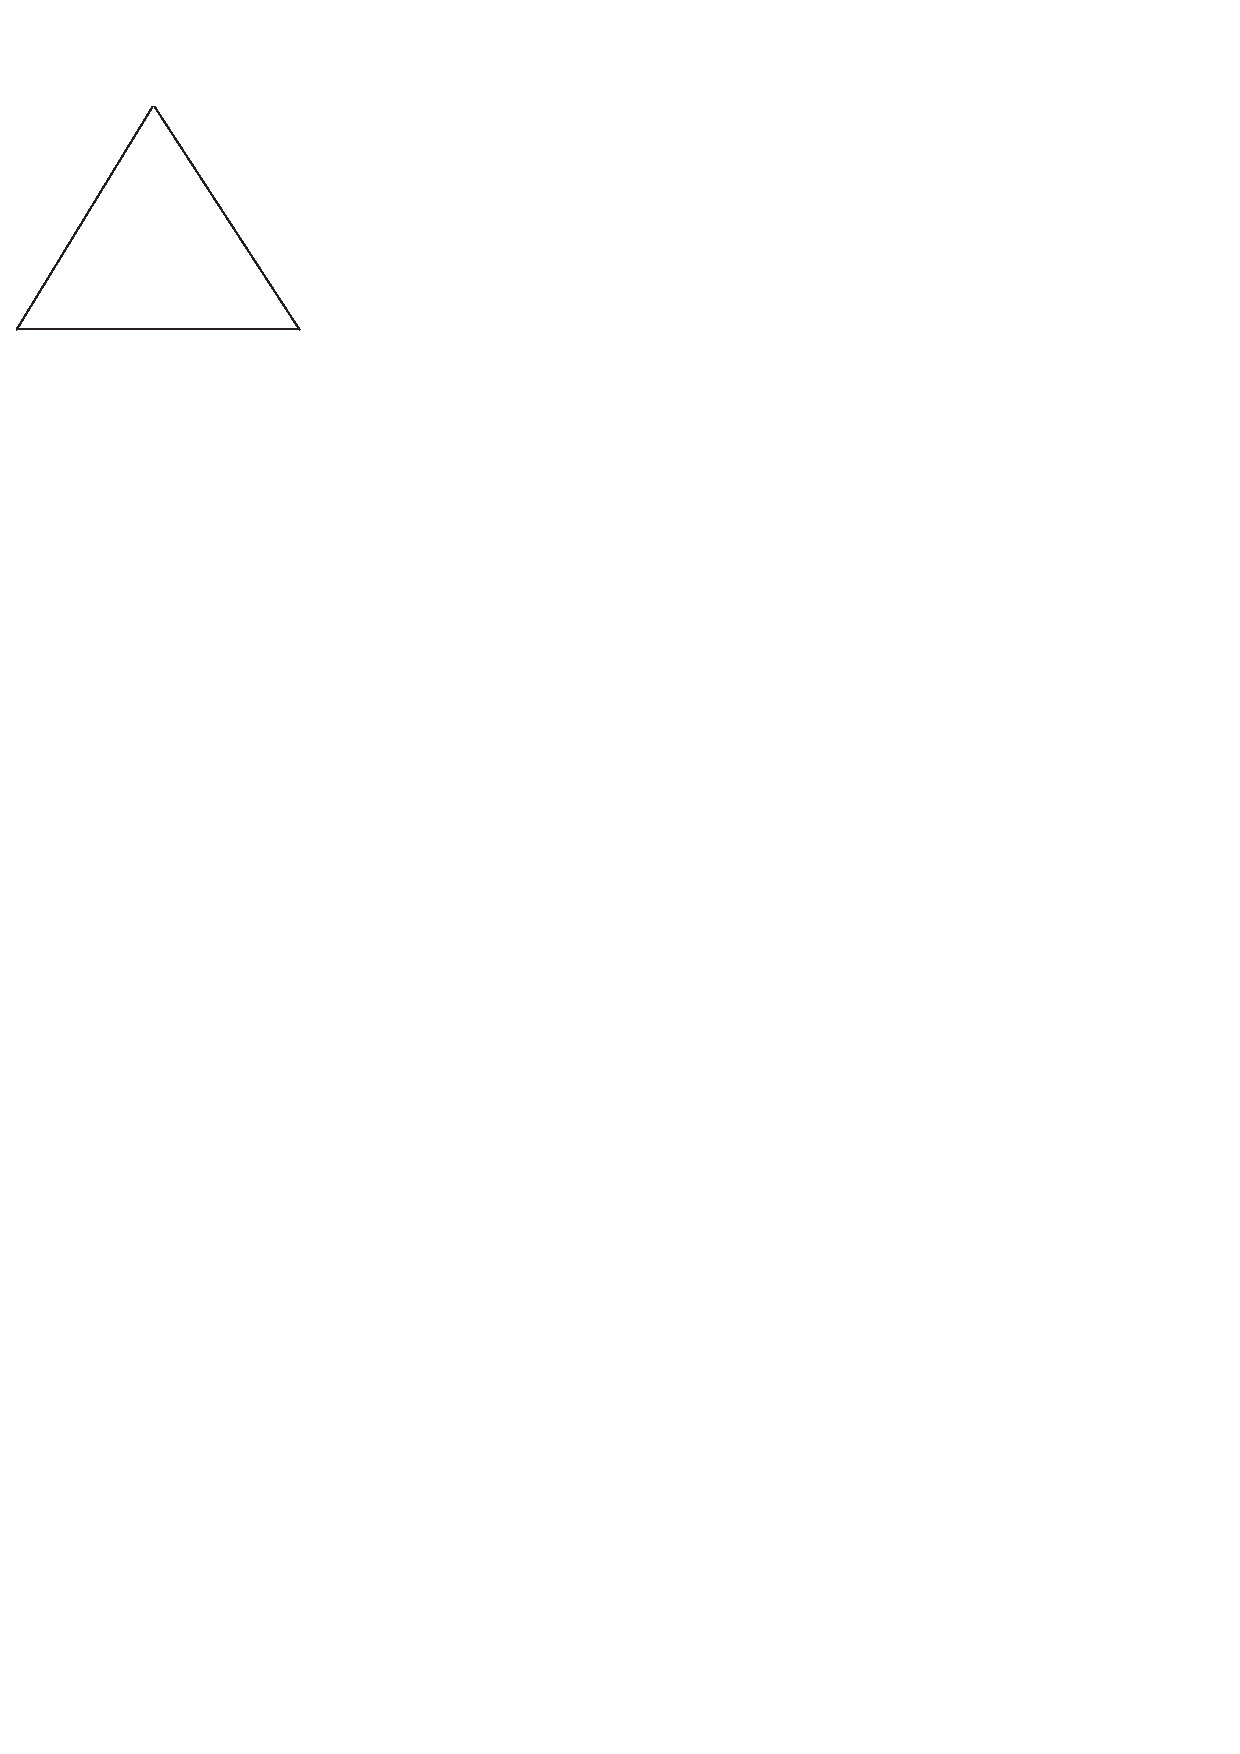
\includegraphics[width=1in]{ch3-triangle.pdf}}\\
%\hbox to 1in{\hfill(c)\hfill}
%\end{gathered}
%\]
%
%\caption{Two rows of graphics: (a)~Square \ (b)~Circle \ (c)~Rectangle }\label{fig:3.1}
%\end{figure}
%

\newpage
Three figures across the page requires fairly small figures to fit within the Graduate School margins.\\

%
\begin{figure}[!h]%  Fig 3.2		% DVI Version
\[
\begin{gathered}
\hbox to 1in{
\includegraphics[width=1in]{ch3-square.ps}}
  \quad
\hbox to 1in{
\includegraphics[width=1in]{ch3-square.ps}}
  \quad
\hbox to 1in{
\includegraphics[width=1in]{ch3-square.ps}}\\[-10pt]
\hbox to 1in{\hfill(a)\hfill}    \quad 
  \hbox to 1in{\hfill(b)\hfill}  \quad 
  \hbox to 1in{\hfill(c)\hfill}
\end{gathered}
\]
%
\vskip 12pt			% vertical space between rows
%
\[
\begin{gathered}
\hbox to 1in{
\includegraphics[width=1in]{ch3-circle.ps}}
  \quad
\hbox to 1in{
\includegraphics[width=1in]{ch3-circle.ps}}
  \quad
\hbox to 1in{
\includegraphics[width=1in]{ch3-circle.ps}}\\[-10pt]
\hbox to 1in{\hfill(d)\hfill}    \quad 
  \hbox to 1in{\hfill(e)\hfill}  \quad 
  \hbox to 1in{\hfill(f)\hfill}
\end{gathered}
\]
%
\vskip 12pt			% vertical space between rows
%
\[
\begin{gathered}
\hbox to 1in{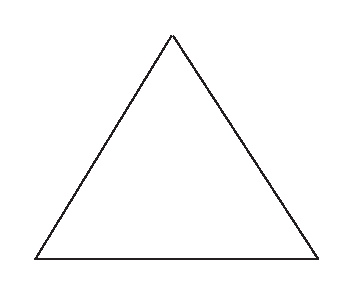
\includegraphics[width=1in]{ch3-triangle.ps}}
  \quad
\hbox to 1in{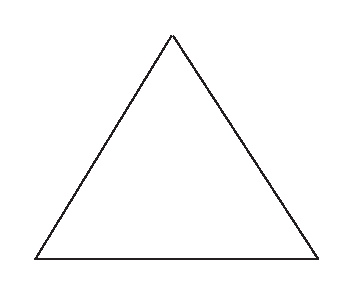
\includegraphics[width=1in]{ch3-triangle.ps}}
  \quad
\hbox to 1in{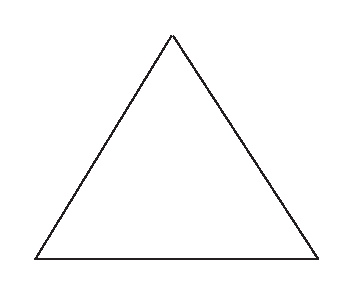
\includegraphics[width=1in]{ch3-triangle.ps}}\\[-10pt]
\hbox to 1in{\hfill(g)\hfill}    \quad 
  \hbox to 1in{\hfill(h)\hfill}  \quad 
  \hbox to 1in{\hfill(i)\hfill}
\end{gathered}
\]
%
\caption{Three rows of graphics: (a)--(c) Squares. \ (d)--(f)~Circles. \ (g)--(i)~Ovals.}\label{fig:3.2}
\end{figure}
%

%
%\begin{figure}[!h]%  Fig 3.2		% PDF Version
%\[
%\begin{gathered}
%\hbox to 1in{
\includegraphics[width=1in]{ch3-square.pdf}}
%  \quad
%\hbox to 1in{
\includegraphics[width=1in]{ch3-square.pdf}}
%  \quad
%\hbox to 1in{
\includegraphics[width=1in]{ch3-square.pdf}}\\[-10pt]
%\hbox to 1in{\hfill(a)\hfill}    \quad 
%  \hbox to 1in{\hfill(b)\hfill}  \quad 
%  \hbox to 1in{\hfill(c)\hfill}
%\end{gathered}
%\]
%%
%\vskip 12pt			% vertical space between rows
%%
%\[
%\begin{gathered}
%\hbox to 1in{
\includegraphics[width=1in]{ch3-circle.pdf}}
%  \quad
%\hbox to 1in{
\includegraphics[width=1in]{ch3-circle.pdf}}
%  \quad
%\hbox to 1in{
\includegraphics[width=1in]{ch3-circle.pdf}}\\[-10pt]
%\hbox to 1in{\hfill(d)\hfill}    \quad 
%  \hbox to 1in{\hfill(e)\hfill}  \quad 
%  \hbox to 1in{\hfill(f)\hfill}
%\end{gathered}
%\]
%%
%\vskip 12pt			% vertical space between rows
%%
%\[
%\begin{gathered}
%\hbox to 1in{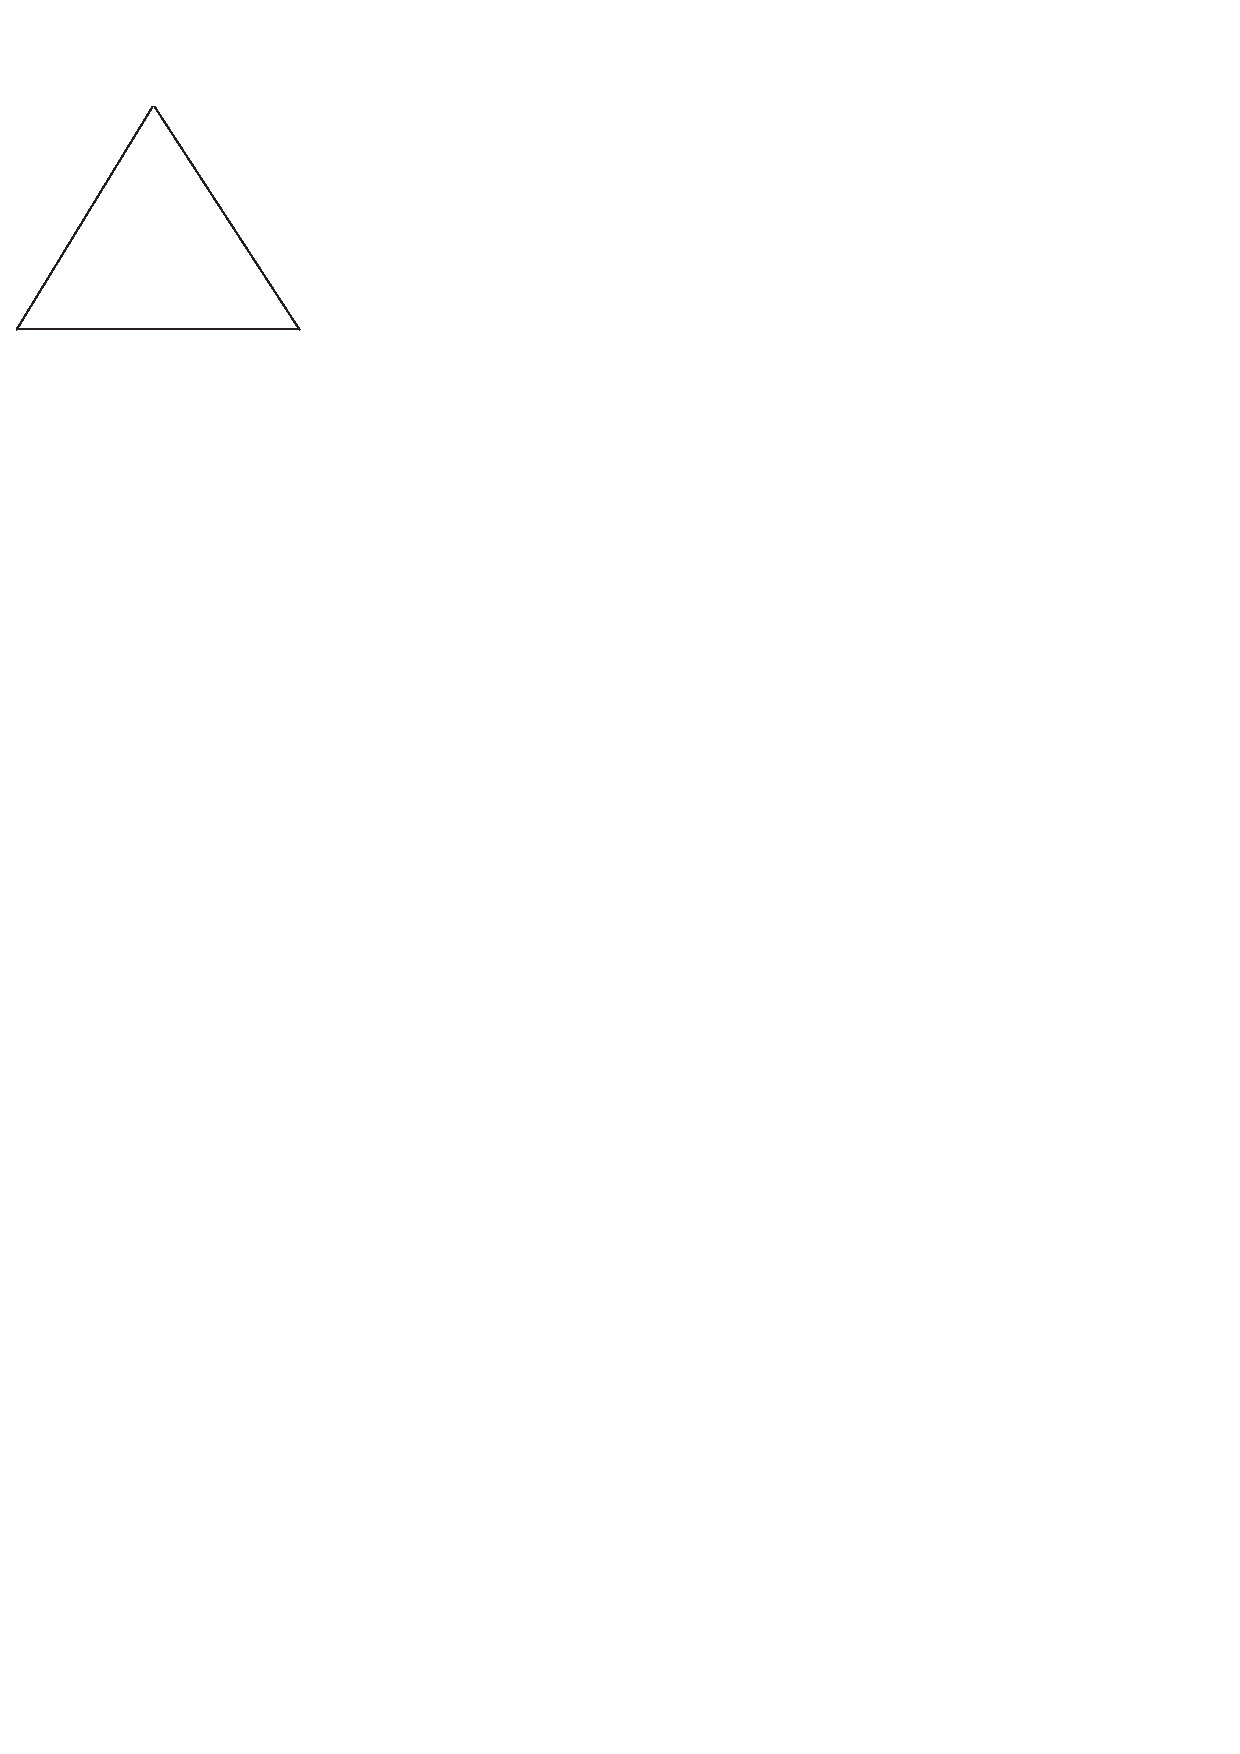
\includegraphics[width=1in]{ch3-triangle.pdf}}
%  \quad
%\hbox to 1in{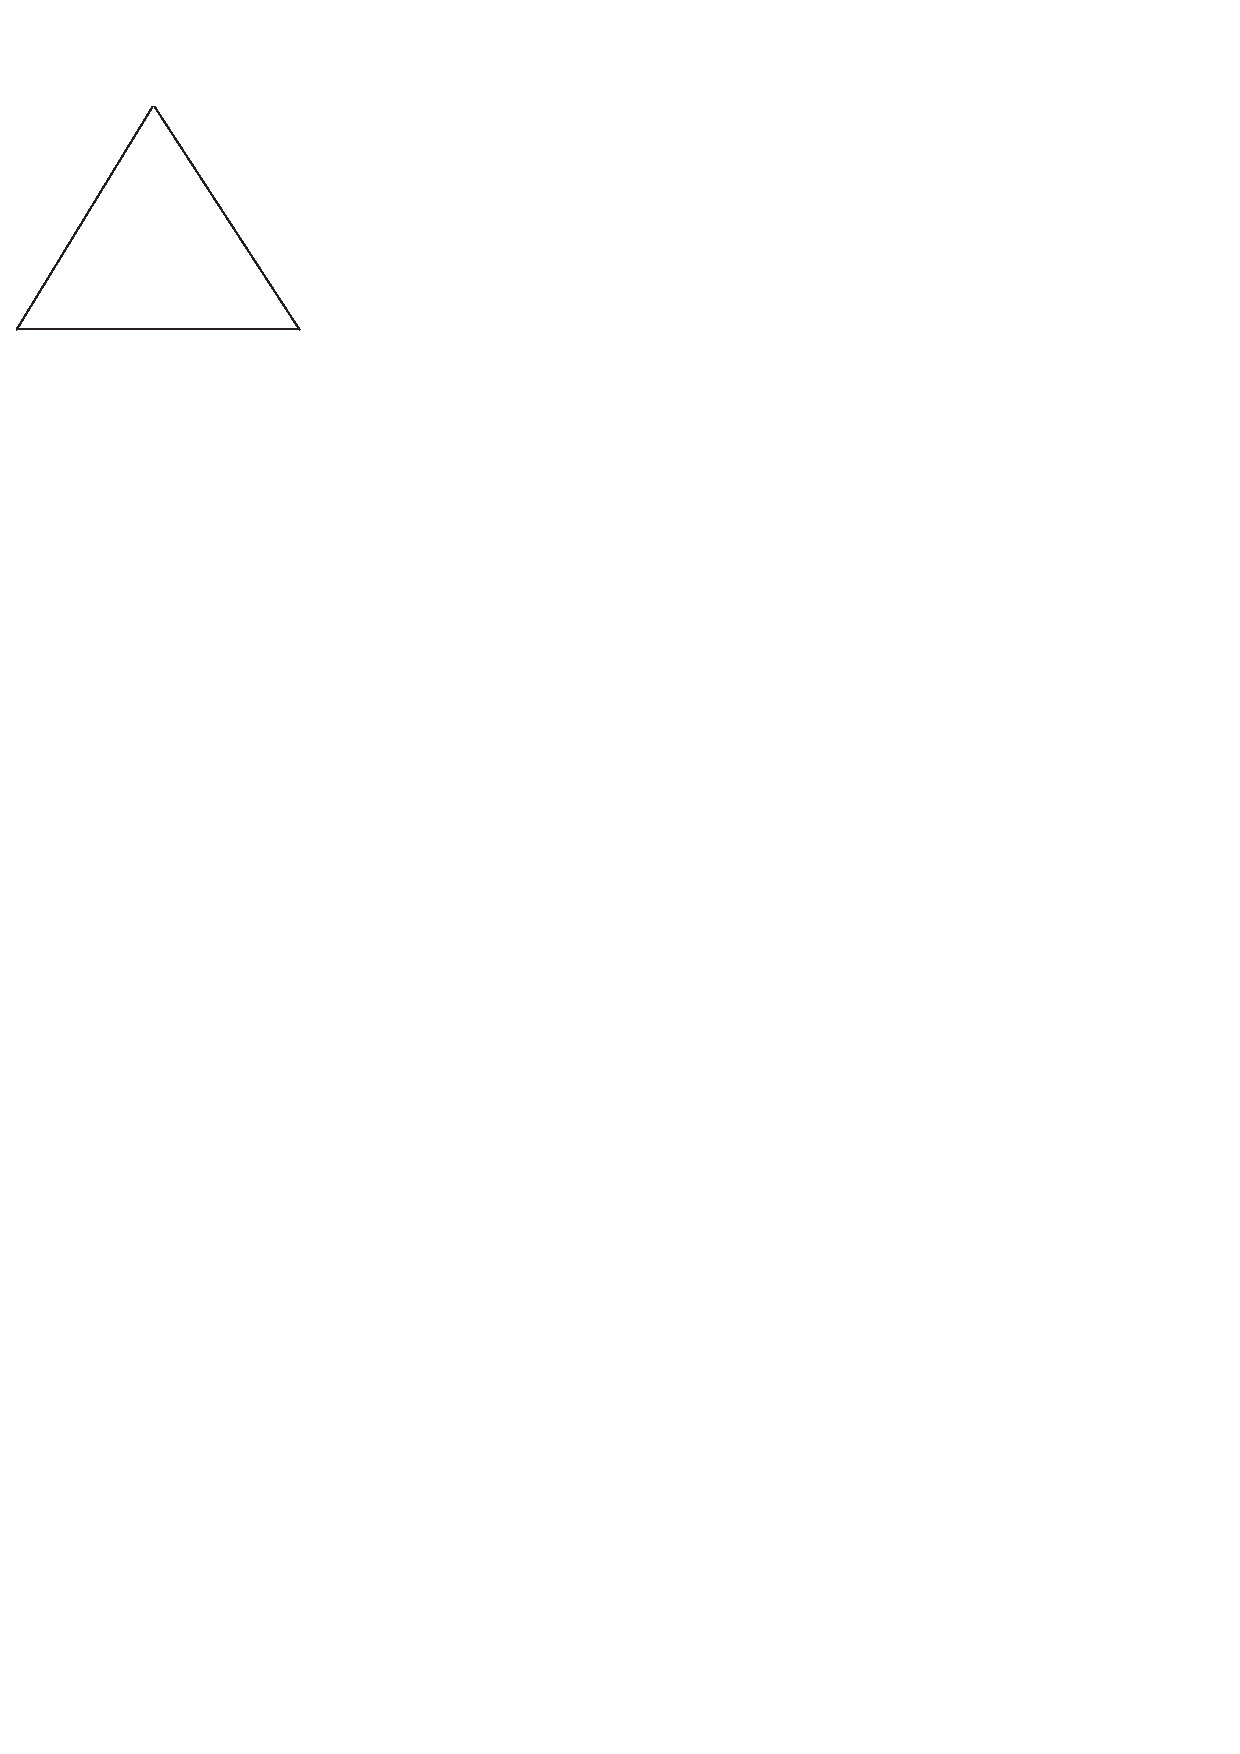
\includegraphics[width=1in]{ch3-triangle.pdf}}
%  \quad
%\hbox to 1in{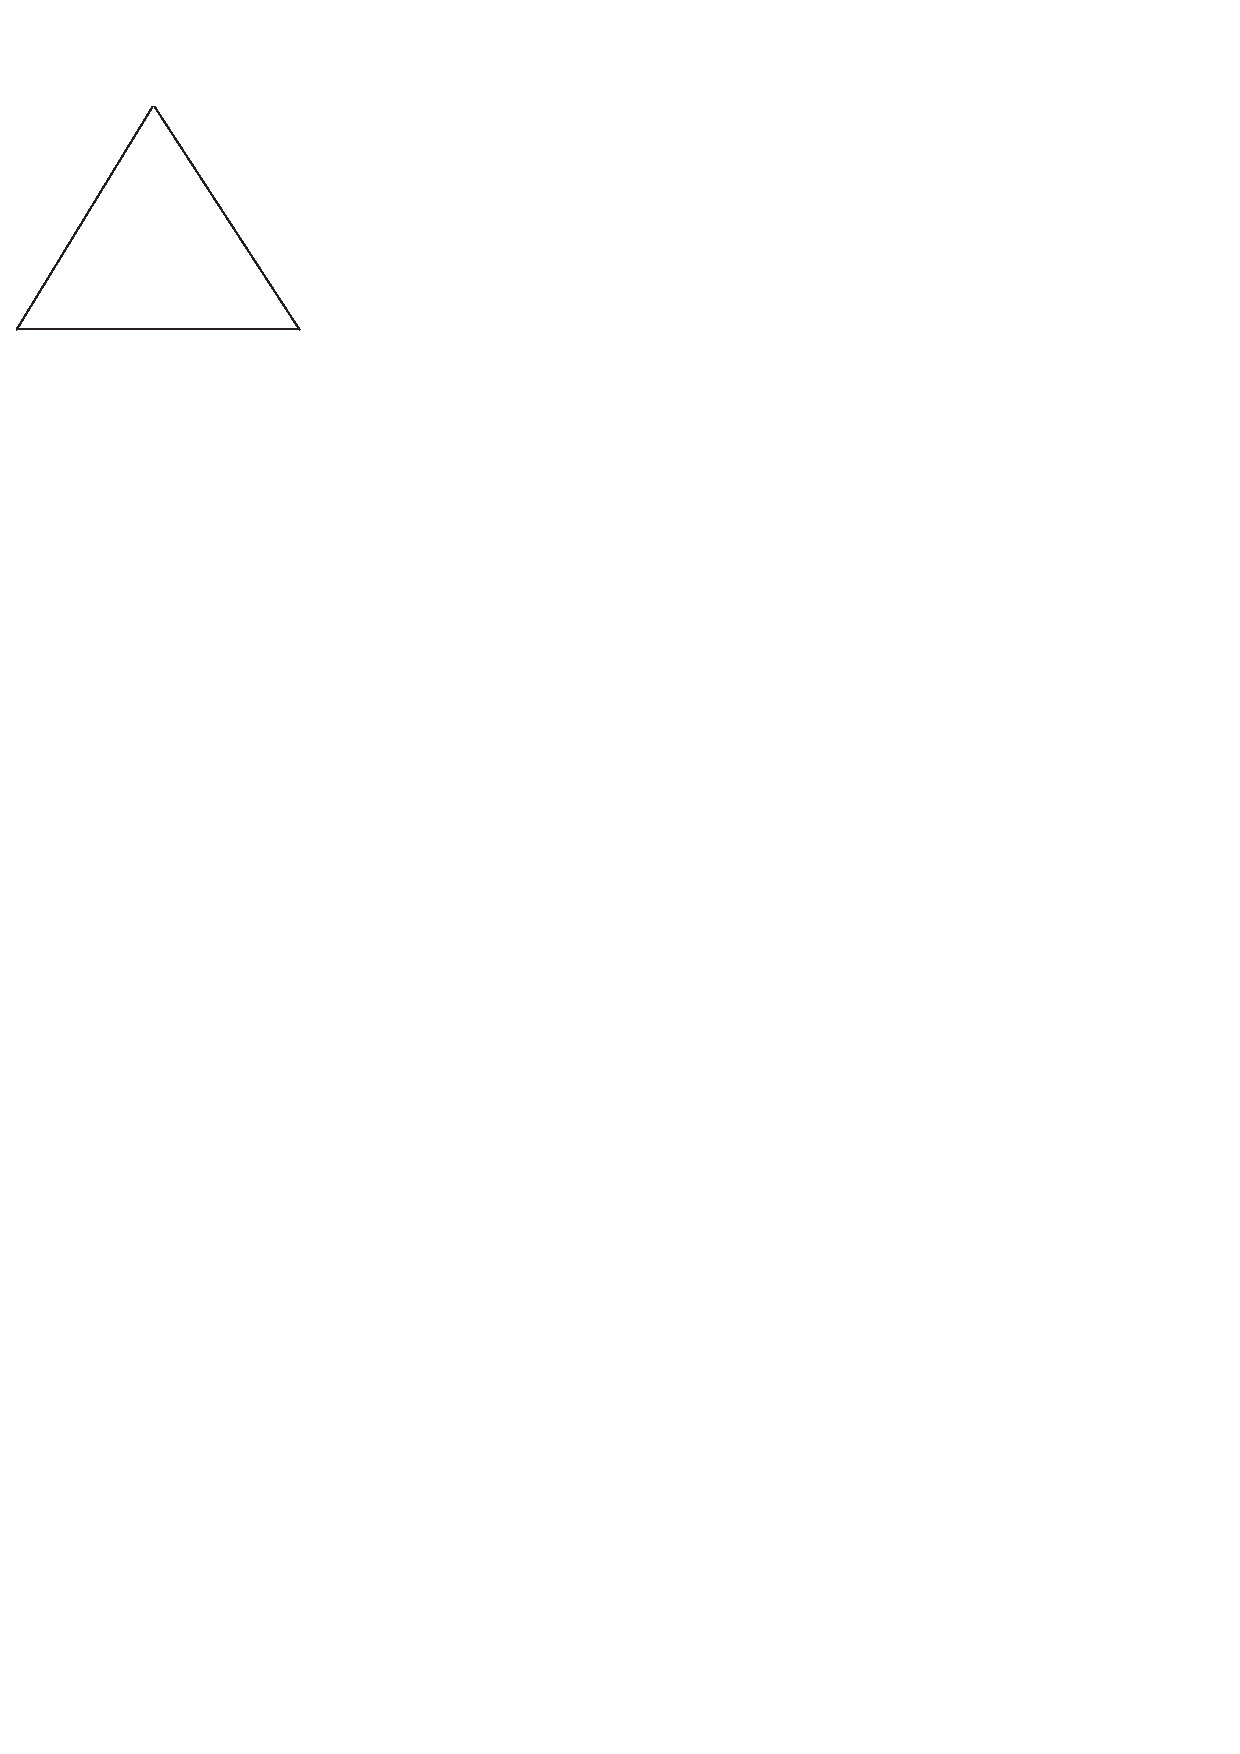
\includegraphics[width=1in]{ch3-triangle.pdf}}\\[-10pt]
%\hbox to 1in{\hfill(g)\hfill}    \quad 
%  \hbox to 1in{\hfill(h)\hfill}  \quad 
%  \hbox to 1in{\hfill(i)\hfill}
%\end{gathered}
%\]
%%
%\caption{Three rows of graphics: (a)--(c) Squares. \ (d)--(f)~Circles. \ (g)--(i)~Ovals.}\label{fig:3.2}
%\end{figure}
%

\newpage
The verbatim environment can be useful when using data from a spreadsheet as is done below. \\

\begin{figure}[h]
\baselineskip=14pt
\begin{verbatim}
   X,TRUE_SUR,MSE SIM,MSE ZHAO,MSE JIAN,MSE PZHAO,MSE PJIAN
   0.0  0.7520  0.03864  0.01407  0.01407  0.01180  0.01223
   4.0  0.7273  0.04079  0.01675  0.01675  0.01479  0.01551
   8.0  0.7035  0.04203  0.01923  0.01923  0.01675  0.01817
  12.0  0.6524  0.04581  0.02157  0.02135  0.01932  0.02043
  16.0  0.6029  0.05146  0.02345  0.02266  0.02304  0.02320
  20.0  0.5551  0.05343  0.02498  0.02393  0.02627  0.02509
  24.0  0.5089  0.05449  0.02677  0.02453  0.02936  0.02641
  28.0  0.4641  0.05706  0.02901  0.02442  0.03315  0.02722
  32.0  0.4209  0.05719  0.02910  0.02341  0.03558  0.02776
  36.0  0.3790  0.05656  0.02974  0.02229  0.03745  0.02667
  40.0  0.3385  0.05518  0.02940  0.02119  0.03864  0.02618
  44.0  0.2994  0.05344  0.02989  0.02054  0.03928  0.02531
  48.0  0.2615  0.04950  0.02803  0.01906  0.03855  0.02414
  52.0  0.2249  0.04582  0.02712  0.01812  0.03849  0.02229
  56.0  0.1895  0.04101  0.02454  0.01578  0.03632  0.01918
  60.0  0.1552  0.03564  0.02282  0.01315  0.03372  0.01629
  64.0  0.1220  0.03216  0.02124  0.00997  0.03188  0.01391
  68.0  0.0900  0.02420  0.01730  0.00688  0.02551  0.01070
  72.0  0.0590  0.01592  0.01254  0.00363  0.01811  0.00622
  76.0  0.0290  0.00865  0.00838  0.00110  0.00886  0.00368
\end{verbatim}
\caption{Use of verbatim environment}
\end{figure}

On the following page is an example of how to rotate text  that is too long to fit within the horizontal margins that are required.

%%%%%%%%%%%%%%%%%%%%%%%%%%%%%%%%%%%%%%%%%%%%%%%%
%%  Sample ROTATION OF TEXT
%%%%%%%%%%%%%%%%%%%%%%%%%%%%%%%%%%%%%%%%%%%%%%%%

\begin{figure}[h]   % again, the "h" says to put it here
\begin{center}
\leavevmode
%\hbox to 1in{}
\rotatebox{90}{\scriptsize
$
\begin{gathered}
A =
\begin{pmatrix}
-(\hat\theta_{D_1}(3;1)-\hat\theta_{D_1}(1;1)) & 0 & 0 & \cdots & 0 & 0 \\
(\hat\theta_{D_1}(3;1)-\hat\theta_{D_1}(1;1)) & -(\hat\theta_{D_2}(3;1)-\hat\theta_{D_2}(1;1)) & 0 & \cdots & \cdots & 0 \\
0 & (\hat\theta_{D_2}(3;1)-\hat\theta_{D_2}(1;1)) & -(\hat\theta_{D_3}(3;1)-\hat\theta_{D_3}(1;1)) & \ddots & \cdots & 0 \\
\vdots & \ddots & \ddots & \ddots & \ddots & 0 \\
0 & \cdots & 0 & 0 & (\hat\theta_{D_{n-1}}(3;1)-\hat\theta_{D_{n-1}}(1;1)) & -(\hat\theta_{D_n}(3;1)-\hat\theta_{D_n}(1;1)) \\
0 & 0 & 0 & 0 & 0 & (\hat\theta_{D_n}(3;1)-\hat\theta_{D_n}(1;1)) 
\end{pmatrix},  %\hbox to .3in{} 
	\\[40pt]
\begin{pmatrix}
A_1 \\
A_2 \\
\vdots \\
A_n \\
\end{pmatrix},   
\end{gathered}$
}
\caption{Matrix Rotated 90 degrees.}
\end{center}
\end{figure}

\baselineskip=24pt
